\subsection{BÀI TẬP TRẮC NGHIỆM}
\ind{PHẦN I.} \inden{Câu trắc nghiệm nhiều phương án lựa chọn. Mỗi câu hỏi học sinh chỉ chọn một phương án.}\\
\setcounter{ex}{0}
\Opensolutionfile{ans}[ans/1H7-B5-1]
\begin{ex}%Câu 1:%[1H8N7-1]
	Cho khối chóp có diện tích đáy $B$ và chiều cao $h$. Thể tích của khối chóp đã cho bằng
	\choice
	{\True $V=\dfrac{1}{3}Bh$}
	{$V=Bh$}
	{$V=\dfrac{2}{3}Bh$}
	{$V=\dfrac{1}{3}B^2h$}
	\loigiai{
		Thể tích hình chóp là $V=\dfrac{1}{3}Bh$.}
\end{ex}
%-------------------------------------------
\begin{ex}%Câu 2:%[1H8N7-1]
	Cho khối chóp có diện tích đáy $B$ và thể tích bằng $V$. Chiều cao của khối chóp đã cho là
	\choice
	{$h=\dfrac{1}{3}V\cdot B$}
	{\True $h=\dfrac{3V}{B}$}
	{$h=\dfrac{V}{3B}$}
	{$h=\dfrac{V}{B}$}
	\loigiai{
		%Chọn B
		Thể tích khối chóp $V=\dfrac{1}{3}B\cdot h\Rightarrow h=\dfrac{3V}{B}$.
	}
\end{ex}
%-------------------------------------------
\begin{ex}%Câu 3:%[1H8N7-1] 
	Cho khối chóp có diện tích đáy $B=8a^2$ và chiều cao $h=a$. Thể tích của khối chóp đã cho bằng
	\choice
	{$4a^3$}
	{\True $\dfrac{8}{3}a^3$}
	{$8a^3$}
	{$\dfrac{4}{3}a^3$}
	\loigiai{
		%Chọn B
		Thể tích khối chóp $V=\dfrac{1}{3}B\cdot h$ = $\dfrac{1}{3}8a^2\cdot a =\dfrac{8}{3}a^3$.
	}
\end{ex}
%-------------------------------------------
\begin{ex}%Câu 4:%[1H8N7-1] 
	Cho khối chóp có chiều cao bằng $a$ và đáy là hình vuông có cạnh bằng $3a$. Thể tích của khối chóp đã cho bằng
	\choice
	{\True $3a^3$}
	{$9a^3$}
	{$6a^3$}
	{$27a^3$}
	\loigiai{
		%Chọn A
		Thể tích của khối chóp đã cho là $V=\dfrac{1}{3}B\cdot h=\dfrac{1}{3}\left( 3a \right)^2\cdot a=3a^3$.
	}
\end{ex}
%-------------------------------------------
\begin{ex}%Câu 5:%[1H8N7-1] 
	Cho khối lăng trụ có diện tích đáy $B$ và chiều cao $h$. Thể tích của khối lăng trụ đã cho bằng
	\choice
	{$V=\dfrac{1}{3}Bh$}
	{\True $V=Bh$}
	{$V=\dfrac{2}{3}Bh$}
	{$V=\dfrac{1}{3}B^2h$}
	\loigiai{
		Thể tích của khối lăng trụ có diện tích đáy $B$ và chiều cao $h$ là $V=Bh$.	
	}
\end{ex}
%-------------------------------------------
\begin{ex}%Câu 6:%[1H8N7-1] 
	Cho khối lăng trụ có diện tích đáy $B$ và thể tích bằng $V$. Chiều cao của khối lăng trụ đã cho bằng
	\choice
	{$h=\dfrac{1}{3}V\cdot B$}
	{$h=\dfrac{3V}{B}$}
	{$h=\dfrac{V}{3B}$}
	{\True $h=\dfrac{V}{B}$}
	\loigiai{
		Thể tích khối lăng trụ $V=B\cdot h\Rightarrow h=\dfrac{V}{B}$.
	}
\end{ex}
%-------------------------------------------
\begin{ex}%Câu 7:%[1H8N7-1] 
	Cho khối lăng trụ có diện tích đáy $B=7a^2$ và chiều cao $h=2a$. Thể tích khối lăng trụ đã cho bằng  
	\choice
	{$\dfrac{14}{2}a^3$}
	{$\dfrac{14}{3}a^3$}
	{\True $14a^3$}
	{$7a^3$}
	\loigiai{
		Thể tích khối lăng trụ đã cho là $V=B\cdot h=7a^2\cdot 2a=14a^3$.
	}
\end{ex}
%-------------------------------------------
\begin{ex}%Câu 8:%[1H8B7-5] 
	Thể tích của khối lập phương cạnh $3a$ bằng
	\choice
	{$a^3$}
	{$3a^3$}
	{$9a^3$}
	{\True $27a^3$}
	\loigiai{
		Ta có $V=\left( 3a \right)^3=27a^3$.
	}
\end{ex}
%-------------------------------------------
\begin{ex}%Câu 9:%[1H8B7-5] 
	Thể tích khối hộp chữ nhật có ba kích thước là $a$, $b$, $c$ bằng
	\choice
	{\True $V=abc$}
	{$V=\dfrac{1}{3}abc$}
	{$V=\left( abc \right)^2$}
	{$V=\sqrt{abc}$}
	\loigiai{Thể tích khối hộp chữ nhật có ba kích thước là $a$, $b$, $c$ bằng $V=abc$.}
\end{ex}
%-------------------------------------------
\begin{ex}%Câu 10:%[1H8B7-6] 
	Tổng số mặt của hình chóp cụt có đáy là tam giác đều là
	\choice
	{$4$}
	{$2$}
	{$3$}
	{\True $5$}
	\loigiai{
		Tổng số mặt của hình chóp cụt có đáy là tam giác đều là $5$.	
	}
\end{ex}
%-------------------------------------------
\begin{ex}%Câu 11:%[1H8B7-6] 
	Thể tích khối chóp cụt đều có chiều cao $h$, diện tích hai đáy là $S_1$; $S_2$ bằng
	\choice
	{\True $V=\dfrac{1}{3}h\left( S_1+S_2+\sqrt{S_1\cdot S_2} \right)$}
	{$V=\dfrac{1}{3}h\left( S_1\cdot S_2\cdot \sqrt{S_1\cdot S_2} \right)$}
	{$V=h\left( S_1+S_2+\sqrt{S_1\cdot S_2} \right)$}
	{$V=\dfrac{1}{3}h\left( S_1+S_2+\sqrt{S_1+S_2} \right)$}
	\loigiai{
		Thể tích khối chóp cụt đều có chiều cao $h$, diện tích hai đáy là $S_1$, $S_2$ là 
		$$V=\dfrac{1}{3}h\left( S_1+S_2+\sqrt{S_1\cdot S_2} \right).$$
	}
\end{ex}
%-------------------------------------------
\begin{ex}%Câu 12:%[1H8B7-6]
	Thể tích khối chóp cụt đều có chiều cao $h=a$, diện tích hai đáy là $S_1=a^2$; $S_2=9a^2$ bằng
	\choice
	{$V=4a^3$}
	{\True $V=\dfrac{13a^3}{3}$}
	{$V=a^3$}
	{$V=9a^3$}
	\loigiai{
		%Chọn B
		Ta có $V=\dfrac{1}{3}h\left( S_1+S_2+\sqrt{S_1\cdot S_2} \right)=\dfrac{1}{3}\cdot a\cdot \left( a^2+9a^2+\sqrt{a^2\cdot 9a^2} \right)=\dfrac{13a^3}{3}$.
	}
\end{ex}

\begin{ex}%[2-DTH-14-NINHBINH-19]%[Nguyễn Thế Anh, dự án EX5]%[2H1Y3-2]%Câu 3
	Cho hình chóp $S.ABCD$ có đáy là hình vuông cạnh $a$, cạnh bên $SA\perp (ABCD)$ và $SA=a$. Tính theo $a$ thể tích khối chóp $S.ABCD$.
	\choice
	{\True $\dfrac{a^3}{3}$}
	{$a^3$}
	{$\dfrac{a^3}{6}$}
	{$\dfrac{a^3}{2}$}
	\loigiai{
		\immini[thm]{
			Thể tích khối chóp $S.ABCD$ là $V=\dfrac{1}{3}SA\cdot S_{ABCD}=\dfrac{a^3}{3}$.}{\begin{tikzpicture}[scale=0.5, line join = round, line cap = round]
				\tikzset{label style/.style={font=\footnotesize}}
				\tkzDefPoints{0/0/D,4/0/C,2/2/A}
				\coordinate (B) at ($(A)+(C)-(D)$);
				\coordinate (S) at ($(A)+(0,3)$);
				\tkzDrawPolygon(S,B,C,D)
				\tkzDrawSegments(S,C)
				\tkzDrawSegments[dashed](A,S A,B A,D)
				\tkzDrawPoints(D,C,A,B,S)
				\tkzLabelPoints[above](S)
				\tkzLabelPoints[left](A,D)
				\tkzLabelPoints[right](B,C)
		\end{tikzpicture}}
	}
\end{ex}

\begin{ex}%[Thi thử lần 1, Ngô Sĩ Liên, Bắc Giang 2019]%[Trần Hòa, 12-EX3-2019]%[2H1Y3-2]%Câu 4
	Cho khối chóp $S.ABC$ có đáy là tam giác đều cạnh bằng $a$, $SA=a\sqrt{3}$, cạnh bên $SA$ vuông góc với đáy. Thể tích khối chóp $S.ABC$ bằng
	\choice
	{$\dfrac{a^3}{2}$}
	{\True $\dfrac{a^3}{4}$}
	{$\dfrac{a^3\sqrt{3}}{4}$}
	{$\dfrac{a^3\sqrt{3}}{2}$}
	\loigiai{
		\immini[thm]{Thể tích khối chóp là\\
			$V=\dfrac{1}{3}\cdot SA\cdot S_\text{ABC}=\dfrac{1}{3}\cdot a\sqrt{3} \cdot \dfrac{a^2\sqrt{3}}{4}=\dfrac{a^3}{4}$.}{\begin{tikzpicture}[scale=1]
				\tkzDefPoints{0/0/A, 1/-1/B, 3/0/C}
				\coordinate (S) at ($(A)+(0,2)$);
				\tkzDrawPolygon(S,A,B)
				\tkzDrawSegments[dashed](A,C)
				\tkzDrawSegments(C,B S,C)
				\tkzLabelPoints[below](C, B)
				\tkzLabelPoints[left](A)
				\tkzLabelPoints[above](S)
				\tkzDrawPoints[fill=black](S,A,B,C)
	\end{tikzpicture}}}
\end{ex}


\begin{ex}%[Đề HK1, Sở GD và ĐT Quảng Nam 2017]%[2H1B3]%Câu 9
	Cho hình chóp $S.ABC$ có đáy là tam giác đều cạnh $a$ và thể tích bằng $3a^3$. Tính chiều cao $h$ của khối chóp $S.ABC$.
	\choice
	{\True $h=12\sqrt3 a$}
	{$h=6\sqrt3 a$}
	{$h=4\sqrt3 a$}
	{$h=2\sqrt3 a$}
	\loigiai{\immini[thm]{
			
			Ta có: $S_{\triangle ABC}=\dfrac{a^2\sqrt3}{4}$.\\
			Suy ra: $h=\dfrac{3V_{S.ABC}}{S_{\triangle ABC}}=12\sqrt3a$.}
		{\begin{tikzpicture}[scale=0.5]
				\tkzDefPoints{0/0/A,2/6/S,7/0/C,3/-2/B}
				\coordinate (H) at ($(S)+(0,-6.6)$);
				\tkzDrawSegments(C,B C,S S,A A,B S,B)
				\tkzDrawSegments[dashed](A,C S,H)
				\tkzDrawSegments[dashed](B,C)
				\tkzLabelPoints[below](B)
				\tkzLabelPoints[right](C,H)
				\tkzLabelPoints[left](A)
				\tkzLabelPoints[above](S)
				\tkzMarkRightAngle(S,H,A)
		\end{tikzpicture}}
	}
\end{ex}

\begin{ex}%[Đề thi HK1 An Phước, Ninh Thuận]%[2H1B3]%Câu 10
	Cho hình chóp $S.ABC$ có $V_{S.ABC}=\dfrac{a^3\sqrt{2}}{36}$ và mặt bên $SBC$ là tam giác đều cạnh $a$. Khoảng cách từ $A$ đến $(SBC)$ bằng
	
	\choice
	{$\dfrac{a\sqrt{2}}{9}$}
	{$\dfrac{a\sqrt{6}}{3}$}
	{\True $\dfrac{a\sqrt{6}}{9}$}
	{$\dfrac{a\sqrt{6}}{27}$}
	\loigiai{$d[A;(SBC)]=\dfrac{3V_{S.ABC}}{S_{ABC}}=
		\dfrac{3.\dfrac{a^3\sqrt{2}}{36}}{\dfrac{a^2\sqrt{3}}{4}}=\dfrac{a\sqrt{6}}{9}$.
		
	}
\end{ex}

\begin{ex}%[2H1B3-2]
	Cho khối chóp tam giác đều $S.ABC$ có cạnh đáy bằng $a$, góc giữa cạnh bên và đáy bằng $30^{\circ}$. Thể tích khối chóp $S.ABC$ bằng
	\choice
	{$\dfrac{a^3\sqrt{2}}{18}$}
	{$\dfrac{a^3\sqrt{2}}{36}$}
	{$\dfrac{a^3\sqrt{3}}{18}$}
	{\True $\dfrac{a^3\sqrt{3}}{36}$}
	\loigiai{
		\immini{
			Gọi $H$ là hình chiếu của $S$ lên $(ABC)$. Khối chóp $S.ABC$ đều nên $H$ là trọng tâm của tam giác $ABC$.\\
			Xét tam giác $ABI$ ta có \[AI=\sqrt{AB^2-BI^2}=\sqrt{a^2-\left(\dfrac{a}{2}\right)^2}=\dfrac{a\sqrt {3}}{2}.\]
			Vì $H$ là trọng tâm của tam giác $ABC$ nên \[AH=\dfrac{2}{3}AI=\dfrac{2}{3}\dfrac{a\sqrt {3}}{2}=\dfrac{a\sqrt {3}}{3}.\]
			
		}{
			\begin{tikzpicture}[scale=1,>=stealth, font=\footnotesize, line join=round, line cap=round]
				\tkzDefPoints{0/0/A,1.2/-1.6/B,4.5/0/C}
				\tkzCentroid(A,B,C)\tkzGetPoint{H}
				\coordinate (S) at ($(H)+(0,3.5)$);
				\coordinate (I) at ($(B)!1/2!(C)$);
				\tkzDrawPolygon(A,B,C,S)
				\tkzDrawSegments(S,B)
				\tkzDrawSegments[dashed](I,A A,C S,H)
				\tkzDrawPoints[fill=black](A,B,C,S,H,I)
				\tkzMarkRightAngles[size=0.14](A,I,B S,H,A)
				\tkzLabelPoints[above](S)
				\tkzLabelPoints[below](B,H,I)
				\tkzLabelPoints[left](A)
				\tkzLabelPoints[right](C)
		\end{tikzpicture}}
		\noindent Lại có $AH$ là hình chiếu vuông góc của $SA$ lên $(ABC)$.	Suy ra $\widehat{\left(SA,(ABC)\right)}=\widehat{(SA,AH)}=30^{\circ}$.\\
		Xét tam giác $SAH$ ta có \[SH=\tan 30^{\circ}\cdot AH=\dfrac{\sqrt {3}}{3}\dfrac{a\sqrt {3}}{3}=\dfrac{a}{3}.\]
		Diện tích tam giác $ABC$ là \[S_{ABC}=\dfrac{1}{2}AB\cdot BC=\dfrac{1}{2}\dfrac{a\sqrt {3}}{2}a=\dfrac{a^2\sqrt {3}}{4}.\]
		Vậy \[V_{S.ABC}=\dfrac{1}{3}S_{ABC}SH=\dfrac{1}{3}\dfrac{a^2\sqrt{3}}{4}\dfrac{a}{3}=\dfrac{a^3\sqrt{3}}{36}.\]
	}    
\end{ex}  

\begin{ex}%[2H1Y3-2]%
	Cho hình lăng trụ đứng có diện tích đáy là $\sqrt{3} a^2 $, độ dài cạnh bên là $ a\sqrt{2}$. Khi đó thể tích của khối lăng trụ bằng
	\choice
	{$\sqrt{2}a^3$}
	{\True $\sqrt{6}a^3$}
	{$\dfrac{\sqrt{6}a^3}{3}$}
	{$\sqrt{3}a^3$}
	\loigiai
	{
		Thể tích của khối lăng trụ bằng $ V=Bh=\sqrt{3} a^2\cdot a\sqrt{2}=\sqrt{6}a^3 $.
	}
\end{ex}

\begin{ex}%[Kiểm tra HK1, SGD Cần Thơ]%[Nguyễn Văn Nay, 12EX4]%[2H1Y3-2]%
	Cho khối lăng trụ tam giác đều có cạnh đáy bằng $ a\sqrt{2} $ và mỗi mặt bên đều có diện tích bằng $ 4a^2 $. Thể tích của khối lăng trụ đã cho bằng
	\choice
	{\True $a^3\sqrt{6}$}
	{ $\dfrac{2a^3\sqrt{6}}{3}$}
	{ $2a^3\sqrt{6}$}
	{ $\dfrac{a^3\sqrt{6}}{3}$}
	\loigiai{
		\immini{Chiều cao của khối lăng trụ là $ h=\dfrac{4a^2}{a\sqrt{2}}=2\sqrt{2}a$.\\
			Thể tích khối lăng trụ $ V=S_{ABC}\cdot h=\dfrac{2a^2\sqrt{3}}{4}\cdot 2\sqrt{2}a=a^3\sqrt{6} $.}{\begin{tikzpicture}[scale=0.6, font=\footnotesize, line join=round, line cap=round, >=stealth]
				\tkzDefPoints{0/0/A,1.1/-1.5/B,3.5/0/C}
				\coordinate (A') at ($(A)+(0,3.2)$);
				\tkzDefPointsBy[translation=from A to A'](B,C){B'}{C'}
				\tkzDrawPolygon(A,B,C,C',B',A')
				\tkzDrawSegments(A',C' B',B)
				\tkzDrawSegments[dashed](A,C)
				\tkzDrawPoints[fill=black,size=4](A,C,B,A',B',C')
				\tkzLabelPoints[below](B)
				\tkzLabelPoints[left](A',A)
				\tkzLabelPoints[right](C',C)
				\tkzLabelPoints[left](B')
		\end{tikzpicture}}
	}
\end{ex}

\begin{ex}%[HK1, Sở GD và ĐT - Đà Nẵng, 2020-2021]%[Lê Vũ Hải, 12EX4]%[2H1B3-2]%
	Cho hình lăng trụ đứng $ABC.A'B'C'$ có đáy là tam giác đều cạnh $a$ và $A'C$ tạo với mặt phẳng đáy một góc $60^{\circ}$. Thể tích khối lăng trụ $ABC.A'B'C'$ bằng
	\choice
	{$\dfrac{a^3}{4}$}
	{$\dfrac{3a^3}{8}$}
	{$\dfrac{3a^3}{2}$}
	{\True $\dfrac{3a^3}{4}$}
	\loigiai{
		\immini{
			Ta có $\left(A'C;(ABC)\right)=\left(A'C;AC\right)=\widehat{A'CA} \Rightarrow \widehat{A'CA}=60^{\circ}$.\\
			$AA'= AC \tan \widehat{A'CA} = a \tan 60^{\circ}=a\sqrt{3}$.\\
			$V = AA' \cdot S_{ABC} = \dfrac{3a^3}{4}$.
		}{
			\begin{tikzpicture}[scale=0.5, font=\footnotesize, line join=round, line cap=round, >=stealth]
				\tkzDefPoints{0/0/A', 5/0/B', 2/-2/C', 0/-5/A}
				\tkzDefPointBy[translation=from A' to A](B') \tkzGetPoint{B}
				\tkzDefPointBy[translation=from A' to A](C') \tkzGetPoint{C}
				\tkzDrawPoints[fill=black](A,A',B',C',B,C)
				\tkzDrawSegments(A',C' A',B' B',C' A',A B',B C',C A,C B,C A',C)
				\tkzDrawSegments[dashed](A,B)
				\tkzLabelPoints[left](A)
				\tkzLabelPoints[above](A',B')
				\tkzLabelPoints[below](B,C)
				\tkzLabelPoints[below right](C')
			\end{tikzpicture}
		}
	}
\end{ex}

\begin{ex}%[Dự án Tex Strong lần 2, Kiều Ngân]%[2H1B3-2]%
	Cho lăng trụ đứng $ABC.A'B'C'$ có đáy là tam giác vuông cân tại $B$, $AC=a\sqrt{2}$, biết góc giữa $(A'BC)$ và đáy bằng $60^\circ$. Thể tích của khối lăng trụ đã cho bằng
	\choice
	{$\dfrac{a^3\sqrt{6}}{6}$}
	{\True $\dfrac{a^3\sqrt{3}}{2}$}
	{$\dfrac{a^3\sqrt{3}}{3}$}
	{$\dfrac{a^3\sqrt{3}}{6}$}
	\loigiai{
		\begin{center}
			\begin{tikzpicture}[line join=round, line cap=round,>=stealth,scale=0.8]
				\tikzset{label style/.style={font=\footnotesize}}
				\coordinate (A) at (0,0);
				\coordinate (B) at (2.5,-1.5);
				\coordinate (C) at (4,0);
				\coordinate (A') at ($(A)+(0,4)$);
				\coordinate (B') at ($(A')+(B)-(A)$);
				\coordinate (C') at ($(A')+(C)-(A)$);
				\draw (A)--(B)--(C)--(C')--(A')--(B')--(C') (A)--(A')--(B)--(B');
				\draw [dashed] (A)--(C)--(A');
				\foreach \d/\g in {A/180, B/-90,C/0,A'/180,B'/90,C'/0}{
					\draw[fill=black](\d) circle (1pt) +(\g:.35)node{$\d$};}
				\foreach \x/\y/\z in {A/B/C}\pic[draw,angle radius=1.8mm]{right angle=\x--\y--\z};
				\draw
				pic[draw]{angle = A'--B--A};
				\node at ($(B)+(132:1.2)$){$60^\circ$};
			\end{tikzpicture}
		\end{center}
		Ta có $\heva{&BC\perp AB\\&BC\perp AA'}\Rightarrow BC\perp A'B$.\\
		Do đó góc giữa $(A'BC)$ và $(ABC)$ là góc giữa $A'B$ và $AB$ là $\widehat{A'BA}=60^\circ$.\\
		Vì tam giác $ABC$ vuông cân tại $B$ nên $AB=BC=\dfrac{AC}{\sqrt{2}}=a$.\\
		Tam giác $AA'B$ vuông tại $A$ có $AA'=AB\cdot \tan \widehat{A'BA}=AB\cdot \tan 60^\circ=a\sqrt{3}$.\\
		Vậy thể tích khối lăng trụ $ABC.A'B'C'$ là $$V=AA'\cdot S_{ABC}=a\sqrt{3}\cdot \dfrac{1}{2}a^2=\dfrac{a^3\sqrt{3}}{2}.$$
	}
\end{ex}

\begin{ex}%[Đặng Đức Quý]%[2H1Y3-2]%
	Thể tích của khối lập phương $ABCD.A'B'C'D'$ có $AC'=3a$ bằng
	\choice
	{\True $3\sqrt{3}a^3$}
	{$9a^3$}
	{$\sqrt{3}a^3$}
	{$3a^3$}
	\loigiai{
		\begin{center}
			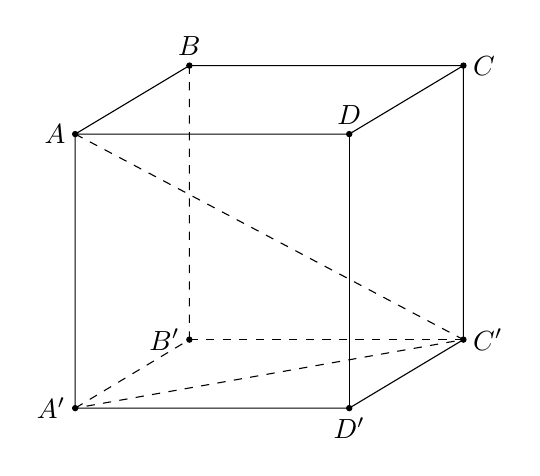
\begin{tikzpicture}[scale=0.58]
				\coordinate[label=left:$A$](A) at (1,5);
				\coordinate[label=above:$B$](B) at (3.5,6.5);
				\coordinate[label=right:$C$](C) at (9.5,6.5);
				\coordinate[label=above:$D$](D) at (7,5);
				\coordinate[label=left:$A'$](A') at (1,-1);
				\coordinate[label=left:$B'$](B') at (3.5,0.5);
				\coordinate[label=right:$C'$](C') at (9.5,0.5);
				\coordinate[label=below:$D'$](D') at (7,-1);
				\fill (A) circle (2pt) (B) circle (2pt) (C) circle (2pt) (D) circle (2pt) (A') circle (2pt) (B') circle (2pt) (C') circle (2pt) (D') circle (2pt);
				\draw (A)--(B)--(C)--(D)--(A)--(A')--(D')--(C')--(C);
				\draw (D)--(D');
				\draw[dashed](B)--(B')--(A');
				\draw[dashed](B')--(C');
				\draw[dashed](A)--(C')--(A');
			\end{tikzpicture}
		\end{center}
		Ta có $AC'=3a$ suy ra độ dài cạnh khối lập phương là $\sqrt{3}a$.\\
		Vậy thể tích của khối lập phương là $V=\left(\sqrt{3}a\right)^3=3\sqrt{3}a^3$.
	}
\end{ex}


\begin{ex}%[Nguyễn Tiến, TEX lần 2]%[2H1B3-2]%
	Cho hình hộp chữ nhật $ABCD.A'B'C'D'$ có $AB=2$ cm, $AD=3$ cm, $AC'=7$ cm. Thể tích của khối hộp $ABCD.A'B'C'D'$ bằng
	\choice
	{$24$ cm$^3$}
	{$42$ cm$^3$}
	{$12$ cm$^3$}
	{\True $36$ cm$^3$}
	\loigiai{
		\begin{center}
			\begin{tikzpicture}[scale=0.4, font=\footnotesize, line join=round, line cap=round, >=stealth]
				\def\bc{4} % cạnh BC
				\def\ba{2} % cạnh BA
				\def\h{3} % đường cao
				\def\gocB{35} % góc B của đáy
				\coordinate[label=below left:$B$] (B) at (0,0);
				\coordinate[label=above left:$A$] (A) at (\gocB:\ba);
				\coordinate[label=below:$C$] (C) at (\bc,0);
				\coordinate[label=right:$D$] (D) at ($(C)-(B)+(A)$);
				\coordinate[label=above left:$A'$] (A') at ($(A)+(90:\h)$);
				\coordinate[label=left:$B'$] (B') at ($(B)-(A)+(A')$);
				\coordinate[label=below right:$C'$] (C') at ($(C)-(A)+(A')$);
				\coordinate[label=right:$D'$] (D') at ($(D)-(A)+(A')$);
				\draw (B')--(B)--(C)--(D)--(D')--(A')--(B')--(C')--(D') (C)--(C')--(A');
				\draw[dashed] (A')--(A)--(D) (A)--(B) (C)--(A)--(C');
				\foreach \diem in {A,B,C,D,A',B',C',D'}\fill (\diem)circle(1.5pt);
			\end{tikzpicture}
		\end{center}
		Trong hình chữ nhật $ABCD$ có $BC=AD=3$ cm.\\
		Nên $AC=\sqrt{AB^2+BC^2}=\sqrt{2^2+3^2}=\sqrt{13}$ cm.\\
		$\Rightarrow A'C'=AC=\sqrt{13}$ cm.\\
		Xét $\triangle AA'C'$ có $AA'=\sqrt{AC'^2-A'C'^2}=\sqrt{49-13}=6 \text{ cm}$.\\
		Vậy thể tích của khối hộp $ABCD.A'B'C'D'$ là
		$$V=AA'\cdot AB\cdot AD=6\cdot 2\cdot 3=36 \text{ cm}^3.$$
	}
\end{ex}

\begin{ex}%[Nguyễn Minh Hiếu]%[2H1B3-2]%
	Cho hình hộp chữ nhật $ABCD.A'B'C'D'$ có $AB=a$, $AC=2a$, tam giác $A'AC$ vuông cân tại $A$. Thể tích khối hộp đã cho bằng
	\choice
	{\True $2\sqrt{3}a^3$}
	{$\dfrac{2\sqrt{3}a^3}{3}$}
	{$\dfrac{2\sqrt{3}a^3}{2}$}
	{$\sqrt{3}a^3$}
	\loigiai{
		Ta có $BC=\sqrt{AC^2-AB^2}=a\sqrt{3}\Rightarrow S_{ABCD}=AB\cdot BC=a^2\sqrt{3}$.\\
		Tam giác $A'AC$ vuông cân tại $A$, suy ra $AA'=AC=2a$.\\
		Vậy thể tích khối hộp chữ nhật là $V=a^2\sqrt{3}\cdot 2a=2a^3\sqrt{3}$.
	}
\end{ex}

\begin{ex}%[2H1K3-2]%câu 64
	Cho hình hộp chữ nhật $ABCD.A'B'C'D'$ có $ AB=AA'=a$, đường chéo $ A'C$ tạo với mặt đáy $(ABCD)$ một góc $\alpha $ thỏa $\cot\alpha=\sqrt{5} $. Thể tích khối hộp đã cho bằng
	\choice
	{\True $ 2a^3$}
	{$\sqrt{5}a^3$}
	{$\dfrac{2a^3}{3}$}
	{$\dfrac{a^3}{\sqrt{5}}$}
	\loigiai{
		\immini{Xác định $\alpha=\left(\widehat{A'C,(ABCD)}\right)=\left(\widehat{A'C,AC}\right)=\widehat{A'CA}$.\\
			Ta có
			\[
			\heva{&AC=AA'\cdot\cot\alpha=a\sqrt{5}\\&AB=AA'=a}\Rightarrow BC=\sqrt{AC^2-AB^2}=2a
			\]
			Vậy $V_{ABCD.A'B'C'D'}=AA'\cdot AB\cdot BC=2a^3$.}{\begin{tikzpicture}[scale=0.8, line join=round, line cap=round]
				\tikzset{label style/.style={font=\footnotesize}}
				\tkzDefPoints{0/0/A,-1.3/-1.1/B,2/-1.1/C}
				\coordinate (D) at ($(A)+(C)-(B)$);
				\coordinate (A') at ($(A)+(0,2.5)$);
				\tkzDefPointsBy[translation=from A to A'](B,C,D){B'}{C'}{D'}
				\tkzDrawPolygon(A',B',B,C,D,D')
				\tkzDrawSegments(B',C' C',D' C,C')
				\tkzDrawSegments[dashed](A,B A,D A,A' A',C A,C)
				\tkzDrawPoints[fill=black,size=4](A,B,D,C,A',B',C',D')
				\tkzLabelPoints[above](A',D')
				\tkzLabelPoints[below](A,B,C)
				\tkzLabelPoints[left](B')
				\tkzLabelPoints[right](C',D)
	\end{tikzpicture}}}
\end{ex}
\Closesolutionfile{ans}

\ind{PHẦN II.} \inden{Câu trắc nghiệm đúng sai. Trong mỗi ý a), b), c), d) ở mỗi câu, học sinh chọn đúng hoặc sai.}\\
\Opensolutionfile{ans}[ans/1H7-B5-2]
\begin{ex}%Câu 1:%[1H8B7-3] 
	Cho khối chóp $S.ABCD$ có đáy $ABCD$ là hình vuông cạnh bằng $2a$, $SA\perp \left( ABCD \right)$, $SA=\dfrac{2a}{\sqrt{3}}$. Các mệnh đề sau đúng hay sai?
	\choiceTF
	{\True Chiều cao của khối chóp $S.ABCD$ bằng $\dfrac{2a\sqrt{3}}{3}$}
	{Diện tích đáy của khối chóp $S.ABCD$ bằng $2a^2$}
	{Chiều cao $AH$ của khối chóp $A.SCD$ bằng $a\sqrt{3}$}
	{Thể tích của khối tứ diện $AHCD$ bằng $\dfrac{a^3\sqrt{3}}{6}$}
	\loigiai{
		\begin{center}
			\begin{tikzpicture}[scale=1, font=\footnotesize, line join=round, line cap=round, >=stealth]
				\path (0,0)coordinate (A)
				(4,0)coordinate (B) 
				(-1.5,-1.7)coordinate (D)
				($(B)+(D)-(A)$)coordinate (C)
				($(A)+(0,3)$)coordinate (S)
				($(S)!0.3!(D)$)coordinate (H);
				\draw (S)--(D)--(C)--(B)--(S)--(C)--(H);
				\draw[dashed] (D)--(A)--(B)(S)--(A)--(H);
				\foreach \x/\y in {S/90,A/180,B/0,C/-45,D/-135,H/150}{\fill (\x) circle (1pt) ($(\x)+(\y:0.3cm)$) node{$\x$};}
				\foreach \a/\b/\c in {S/H/A,S/A/D}{\draw pic[draw,angle radius=2mm] {right angle = \a--\b--\c};}				
			\end{tikzpicture}
		\end{center}
		\begin{itemchoice}
			\itemch  Theo đề $SA\perp \left( ABCD \right)$ nên $SA=\dfrac{2a}{\sqrt{3}}=\dfrac{2a\sqrt{3}}{3}$ là chiều cao của hình chóp. 
			Dó đó mệnh đề đúng.
			\itemch  Diện tích đáy của khối chóp $S.ABCD$ là $S_{ABCD}=\left( 2a \right)^2=4a^2$. 
			Do đó mệnh đề sai.
			\itemch  Gọi $AH$ là đường cao của tam giác $SAD$.\\
			Ta có $\heva{
				& AH\perp SD \\ 
				& AH\perp CD}$\\
			$\Rightarrow AH\perp \left( SCD \right)$ nên $AH$ là đường cao của khối chóp $A.SCD$.\\
			Trong tam giác vuông $SAD$, ta có $\dfrac{1}{AH^2}=\dfrac{1}{SA^2}+\dfrac{1}{AD^2}=\dfrac{3}{4a^2}+\dfrac{1}{4a^2}=\dfrac{1}{a^2}$.\\
			Suy ra $AH=a$.\\
			Do đó mệnh đề sai.
			\itemch Ta có $HD=\sqrt{AD^2-AH^2}=\sqrt{4a^2-a^2}=a\sqrt{3}$ và
			$$V_{C.AHD}=\dfrac{1}{3}S_{ADH}\cdot CD=\dfrac{1}{3}\cdot \dfrac{AH\cdot HD}{2}\cdot CD=\dfrac{1}{3}\cdot \dfrac{a\sqrt{3}\cdot a}{2}\cdot 2a=\dfrac{a^3\sqrt{3}}{3}.$$
			Do đó mệnh đề sai. 
		\end{itemchoice}
	}
\end{ex}
%-------------------------------------------
\begin{ex}%Câu 2:%[1H8B7-5] 
	Cho khối lập phương $ABCD.A'B'C'D'$ có cạnh bằng $a\sqrt{3}$. Các mệnh đề sau đúng hay sai?
	\choiceTF
	{\True Thể tích của khối lập phương $ABCD. A'B'C'D'$ bằng $3a^3\sqrt{3}$}
	{Thể tích của khối lăng trụ $ABD.A'B'D'$ bằng $\dfrac{a^3}{2}$}
	{\True Thể tích của khối tứ diện $B'BAC$ bằng $\dfrac{a^3\sqrt{3}}{2}$}
	{Thể tích của khối tứ diện $B'ACD'$ bằng $\dfrac{3a^3\sqrt{3}}{5}$}
	\loigiai{
		\begin{center}
			\begin{tikzpicture}[scale=0.7, font=\footnotesize, line join=round, line cap=round, >=stealth]
				\path (0,0)coordinate (A)
				(4,0)coordinate (B)
				(1.3,1.7)coordinate (D)
				($(B)+(D)-(A)$)coordinate (C)
				($(A)+(0,3.5)$)coordinate (A')
				($(B)+(A')-(A)$)coordinate (B')
				($(C)+(A')-(A)$)coordinate (C')
				($(D)+(A')-(A)$)coordinate (D');
				\draw (A)--(B)--(C)(A')--(B')--(C')--(D')--(A')--(A) (B)--(B') (C)--(C');
				\draw[dashed] (A)--(D)--(D') (A)--(D)--(C)--(A) (B)--(D);
				\foreach \x/\y in {A/180,B/-45,C/0,D/180,A'/-135,B'/90,C'/0,D'/135}{\fill (\x) circle (1pt) ($(\x)+(\y:0.3cm)$) node{$\x$};}
				
			\end{tikzpicture}
		\end{center}
		\begin{itemchoice}
			\itemch  Gọi $V$ là thể tích của khối lập phương. Ta có $V=\left( a\sqrt{3} \right)^3=3a^3\sqrt{3}$. \\
			Do đó mệnh đề đúng.
			\itemch  Vì khối lăng trụ đứng tam giác $ABD.A'B'D'$ có cùng chiều cao với khối lập phương và có diện tích đáy bằng một nửa diện tích đáy của khối lập phương đã cho nên $V_{ABD.A'B'D'}=\dfrac{V}{2}$.\\
			Do đó mệnh đề sai.
			\itemch  Ta có $V_{B'.BAC}=\dfrac{1}{3}\cdot B’B\cdot \dfrac{BA\cdot BC}{2}=\dfrac{V}{6}=\dfrac{a^3\sqrt{3}}{2}$.\\
			Do đó mệnh đề đúng.
			\itemch  Ta có $V_{B'.BAC}=V_{D'.DAC}=V_{C.C'B'D'}=V_{A.A'B'D'}=\dfrac{V}{6}$ nên ta có $V_{B'.ACD'}=V-4\cdot \dfrac{V}{6}=\dfrac{V}{3}=a^3\sqrt{3}$.\\
			Do đó mệnh đề sai.
		\end{itemchoice}
	}
\end{ex}
%-------------------------------------------
\begin{ex}%Câu 3:%[1H8B7-5] 
	Cho lăng trụ tam giác đều $ABC.A’B’C’$. Biết rằng góc giữa $\left( A’BC \right)$ và $\left( ABC \right)$ là $30^\circ $, tam giác $A’BC$ có diện tích bằng $18$.
	\choiceTF
	{Hình lăng trụ đã cho có đường cao $h=3\sqrt{3}$}
	{\True Diện tích đáy của hình lăng trụ đã cho là $S_{ABC}=9\sqrt{3}$}
	{Thể tích của khối chóp $A'.ABC$ bằng $3\sqrt{3}$}
	{\True Thể tích khối lăng trụ $ABC.A’B’C’$là $V_{ABC.A'B'C'}=27\sqrt{3}$}
	\loigiai{
		\begin{center}
			\begin{tikzpicture}[scale=0.7, font=\footnotesize, line join=round, line cap=round, >=stealth]
				\path (0,0)coordinate (A) 
				(1.8,-1.8)coordinate (B) 
				(5,0)coordinate (C) 
				($(A)+(90:4)$)coordinate (A') 
				($(B)!.5!(C)$)coordinate (M) 
				($(B)+(90:4)$)coordinate (B') 
				($(C)+(90:4)$)coordinate (C') 
				;
				\draw (A')--(B')--(C')--cycle (A')--(A)--(B)--(C)(A')--(B)--(B') (C)--(C');
				\draw[dashed] (A)--(C)--(A') (A)--(M)--(A');
				\foreach \x/\y in {A/180,B/-90,C/0,A'/90,M/-70,B'/-45,C'/0}{\fill (\x) circle (1pt) ($(\x)+(\y:0.3cm)$) node{$\x$};}
				\foreach \a/\b/\c in {A'/M/A}{\draw pic[draw,angle radius=5mm] {angle = \a--\b--\c};}
				\draw (M) node[shift={(-0.8,0.5)}]{$30^\circ$};
			\end{tikzpicture}
		\end{center}
		\begin{itemchoice}
			\itemch  Đặt $AB=x,\left( x>0 \right)$, gọi $M$ là trung điểm $BC$.\\
			Ta có $\heva{&\left( A’BC \right)\cap \left( ABC \right)=BC \\ 
				& AM\perp BC \\ 
				& A’M\perp BC}$\\
			$\Rightarrow \widehat{\left( \left( A’BC \right),\left( ABC \right) \right)}=\widehat{A’MA}=30^\circ $.\\
			Xét $\triangle A’AM$, có $A’M=\dfrac{AM}{\cos 30^\circ} =\dfrac{x\sqrt{3}}{2}\cdot \dfrac{2}{\sqrt{3}}=x$.\\
			$S_{A’BC}=18\Leftrightarrow \dfrac{1}{2}A’M\cdot BC=18\Leftrightarrow x^2=36\Rightarrow x=6$.\\
			Suy ra đường cao của hình lăng trụ là $h=A’A=AM\cdot \tan 30^\circ =\dfrac{6\cdot \sqrt{3}}{2}\cdot \dfrac{1}{\sqrt{3}}=3$.
			\itemch  Tam giác $ABC$ đều nên $S_{ABC}=\dfrac{6^2\cdot \sqrt{3}}{4}=9\sqrt{3}$.
			\itemch  $V_{A'.ABC}=\dfrac{1}{3}A’A\cdot S_{ABC}=\dfrac{1}{3}\cdot 3\cdot 9\sqrt{3}=9\sqrt{3}$.
			\itemch  $V_{ABC.A’B’C’}=A’A.S_{ABC}=3\cdot 9\sqrt{3}=27\sqrt{3}$.
		\end{itemchoice}
	}
\end{ex}
%-------------------------------------------
\begin{ex}%Câu 4:%[1H8B7-2] 
	Cho hình chóp $S.ABC$ có $SA$ vuông góc với đáy, hai mặt phẳng $\left( SAB \right)$ và $\left( SBC \right)$ vuông góc với nhau, $SB=a\sqrt{3}$, góc giữa $SC$ và $\left( SAB \right)$ là $45^\circ $ và $\widehat{ASB}=30^\circ $.
	\choiceTF
	{\True Mặt phẳng $\left( SAB \right)$ vuông góc với mặt phẳng $\left( ABC \right)$}
	{Tam giác $SBC$ vuông cân tại $C$}
	{\True Hai đường thẳng $AB$ và $CB$ vuông góc với nhau}
	{Nếu gọi thể tích khối chóp $S.ABC$ là $V$ thì tỷ số $\dfrac{a^3}{V}$ bằng $\dfrac{3}{8}$}
	\loigiai{
		\begin{center}
			\begin{tikzpicture}[scale=1, font=\footnotesize, line join=round, line cap=round, >=stealth]
				\path (0,0)coordinate (A) 
				(-2.3,-1)coordinate (B) 
				(5,-1)coordinate (C) 
				($(A)+(90:4)$)coordinate (S) 
				;
				\draw (S)--(B)--(C)--cycle;
				\draw[dashed] (S)--(A)--(B)(A)--(C);
				\foreach \x/\y in {S/90,B/-90,C/-90,A/-90}{\fill (\x) circle (1pt) ($(\x)+(\y:0.3cm)$) node{$\x$};}
				\draw (S) node[shift={(-0.23,-1)},scale=0.7]{$30^\circ$}(S) node[shift={(0.3,-0.7)},scale=0.7]{$45^\circ$};
			\end{tikzpicture}
		\end{center}
		\begin{itemchoice}
			\itemch  Theo giả thiết, $\triangle SAB$ vuông tại $A$ có $SB=a\sqrt{3}$, $\widehat{ASB}=30^\circ $. \\
			Khi đó, $SA=SB\cdot \cos 30^\circ =\dfrac{3a}{2}$\\
			và $AB=SB\cdot \sin 30^\circ =\dfrac{a\sqrt{3}}{2}$.\\
			Do $SA\perp \left( ABC \right)$ nên $\left( SAB \right)\perp \left( ABC \right)$. 
			\itemch  Vậy hai mặt phẳng $\left( SBC \right)$ và $\left( ABC \right)$ cùng vuông góc với $\left( SAB \right)$ nên suy ra $BC\perp \left( SAB \right)\Rightarrow \left( SC,\,\left( SAB \right) \right)=\left( SC,\,SB \right)=\widehat{CSB}=45^\circ $.\\
			Suy ra $\triangle SBC$ vuông cân tại $B$.
			\itemch  $\triangle SBC$ vuông cân tại $B \Rightarrow BC=SB=a\sqrt{3}$.\\
			Mặt khác, $BC\perp \left( SAB \right)$\\
			$\Rightarrow CB\perp AB \Rightarrow \triangle ABC$ vuông tại $B$.\\
			Suy ra hai đường thẳng $AB$ và $CB$ vuông góc với nhau.
			\itemch  Khi đó, $S_{\triangle ABC}=\dfrac{1}{2}AB\cdot BC=\dfrac{3a^2}{4}$\\
			Và $V=\dfrac{1}{3}SA\cdot S_{\triangle ABC}=\dfrac{3a^3}{8}$. Vậy tỉ số $\dfrac{a^3}{V}=\dfrac{8}{3}$.
		\end{itemchoice}
	}
\end{ex}
\Closesolutionfile{ans}

\ind{PHẦN III.} \inden{Câu trắc nghiệm trả lời ngắn.}\\
\Opensolutionfile{ans}[ans/1H7-B5-3]
\begin{ex}%Câu 1:%[1H8H7-3] 
	Cho khối chóp $S\cdot ABCD$ có đáy là hình thoi, cạnh bên $SA$ vuông góc với mặt phẳng đáy. Mặt bên $\left( SCD \right)$ tạo với đáy một góc ${60}^{\circ}$, $\widehat{ABC}={60}^{\circ}$, $SA=3\sqrt{3}$. Tính thể tích khối chóp $S\cdot ABCD$.\\
	\shortans[oly]{$18$}
	\loigiai{
		\immini{Gọi $I$ là trung điểm của $CD$.\\
			Vì $ABCD$ là hình thoi có $\widehat{ABC}={60}^{\circ}\Rightarrow \widehat{ADC}=60^{\circ},AD=DC$ $\Rightarrow \triangle ACD$ đều$\Rightarrow AI\perp CD$.\\
			Vậy $\widehat{SIA}$ là góc giữa $\left( SCD \right)$ và $\left( ABCD \right) \Rightarrow \widehat{SIA}={60}^{\circ}$.\\
			Xét tam giác $SAI$ vuông tại $A$ có $\tan \widehat{SIA}=\dfrac{SA}{AI}\Rightarrow AI=\dfrac{SA}{\tan \widehat{SIA}}=\dfrac{3\sqrt{3}}{\tan {60}^{\circ}}=3$.\\
			Tam giác $ACD$ đều có $AI$ là đường cao nên $AI=CD\cdot \dfrac{\sqrt{3}}{2}\Rightarrow CD=\dfrac{2AI}{\sqrt{3}}=\dfrac{2\sqrt{3}\sqrt{3}}{\sqrt{3}}=2\sqrt{3}$.
		}
		{\begin{tikzpicture}[scale=1, font=\footnotesize, line join=round, line cap=round, >=stealth]
				\path (0,0)coordinate (A)
				(4,0)coordinate (D) 
				(-1.3,-1.7)coordinate (B)
				($(B)+(D)-(A)$)coordinate (C)
				($(A)+(0,3)$)coordinate (S)
				($(C)!0.5!(D)$)coordinate (I);
				\draw (I)--(S)--(D)--(C)--(B)--(S)--(C)--(I);
				\draw[dashed] (D)--(A)--(B)(S)--(A)--(I)(A)--(C);
				\foreach \x/\y in {S/90,A/180,B/-90,C/-45,D/0,I/-60}{\fill (\x) circle (1pt) ($(\x)+(\y:0.3cm)$) node{$\x$};}
				\foreach \a/\b/\c in {S/A/D,S/A/B}{\draw pic[draw,angle radius=2mm] {right angle = \a--\b--\c};}
				\foreach \a/\b/\c in {S/I/A}{\draw pic[draw,angle radius=7mm] {angle = \a--\b--\c};}	
				\foreach \a/\b/\c in {S/I/A}{\draw pic[draw,angle radius=6.5mm] {angle = \a--\b--\c};}
				\draw (I) node[shift={(-0.8,0.5)},scale=0.8]{$60^\circ$};			
		\end{tikzpicture}}
		\noindent
		Diện tích $\triangle ACD$ là $S_{\triangle ACD}=\dfrac{1}{2}AI\cdot CD=\dfrac{1}{2}2\sqrt{3}\cdot \sqrt{3}\sqrt{3}=3\sqrt{3}$.\\
		Ta có $S_{ABCD}=2S_{\triangle ACD}=6\sqrt{3}$.\\
		Vậy $V_{S.ABCD}=\dfrac{1}{3}SA\cdot S_{ABCD}=\dfrac{1}{3}\cdot 3\sqrt{3}\cdot 6\sqrt{3}=18$.
	}
\end{ex}

%-------------------------------------------
\begin{ex}%Câu 2:%[1H8H7-4] 
	Cho hình lăng trụ đứng $ABC.A’B’C’$ có tam giác $ABC$ cân, $AB=1$ và $\widehat{BAC}=120^\circ $. Góc giữa mặt phẳng $\left( AB’C’ \right)$ và mặt đáy bằng $60^\circ $. Tính thể tích $V$ khối lăng trụ trên (kết quả làm tròn đến hàng phần trăm).\\
	\shortans[oly]{$0{,}38 $}
	\loigiai{
		\immini{
			Vì tam giác $ABC$ cân và $\widehat{BAC}={120}^{\circ}$ nên tam giác $ABC$ cân tại $A$, do đó $AB=AC=1$.\\
			Diện tích tam giác $ABC$ là $S_{\triangle ABC}=\dfrac{1}{2}AB\cdot AC\cdot \sin A=\dfrac{1}{2}{1^2\cdot \sin {120}^{\circ}}=\dfrac{\sqrt{3}}{4}$.
			Gọi $M$ là trung điểm $B’C’ \Rightarrow A’M'\perp B’C’$.\\
			Vì $AC’=AB’\Rightarrow AM\perp B’C’$.\\
			Khi đó góc giữa mặt phẳng $\left( AB’C’ \right)$ và mặt đáy là $\widehat{AMA’}={60}^{\circ}$.\\
			Ta có $A’M=A’B’\cos \widehat{B’A’M}=1\cdot \cos {60}^{\circ}=\dfrac{1}{2}$.\\
			Từ đó $AA’=A’M\tan \widehat{AMA’}=\dfrac{1}{2}\tan {60}^{\circ}=\dfrac{\sqrt{3}}{2}$.\\
			Vậy $V_{ABC\cdot A’B’C’}=AA’\cdot S_{\triangle ABC}=\dfrac{\sqrt{3}}{2}\cdot \dfrac{1^2\sqrt{3}}{4}=\dfrac{3}{8}$.
		}
		{\begin{tikzpicture}[scale=1, font=\footnotesize, line join=round, line cap=round, >=stealth]
				\path (0,0)coordinate (A)
				(3,2)coordinate (B) 
				(4,0)coordinate (C)
				($(A)+(0,-4)$)coordinate (A')
				($(B)+(0,-4)$)coordinate (B')
				($(C)+(0,-4)$)coordinate (C')
				($(C')!0.5!(B')$)coordinate (M)		
				;
				\draw (A)--(B)--(C)--cycle (C')--(A)--(A')--(C')--(C);
				\draw[dashed] (A)--(M)--(A')--(B')--(C')(B)--(B')(A)--(B');
				\foreach \x/\y in {A/180,B/90,C/0,A'/-90,B'/0,C'/-90,M/30}{\fill (\x) circle (1pt) ($(\x)+(\y:0.3cm)$) node{$\x$};}
				\foreach \a/\b/\c in {A/M/A'}{\draw pic[draw,angle radius=6.5mm] {angle = \a--\b--\c};}
		\end{tikzpicture}}
	}
\end{ex}

%-------------------------------------------
\begin{ex}%Câu 3:%[1H8H7-6] 
	Bạn Mi muốn làm các viên nước đá có dạng khối chóp cụt tứ giác đều có đáy lớn bằng $3$ cm, đáy nhỏ bằng $1{,}5$ cm và cao $3$ cm bằng cách dùng khay đá, mỗi khay sẽ tạo được $6$ viên đá. Hỏi bạn An cần ít nhất bao nhiêu khay để chứa đồng thời 2 lít nước? \\
	\shortans[oly]{$22 $}
	\loigiai{
		Ta có $2\, \mathrm{l}=2000$ cm$^3$. Thể tích mỗi viên đá là
		$$V=\dfrac{1}{3}\cdot h\cdot \left( S+S'+\sqrt{S\cdot S'} \right)=\dfrac{1}{3}\cdot 3\cdot \left( 3^2+1{,}5^2+\sqrt{3^2\cdot 1{,}5^2} \right)=\dfrac{63}{4} \mathrm{cm}^3.$$
		Từ $2$ lít nước có thể tạo ra số viên đá là $\dfrac{2000}{\dfrac{63}{4}}\,\approx 127$ (viên).\\
		Ta có $127\,: 6\approx 21,2$ (khay đá).\\
		Vậy cần ít nhất $22$ khay nước để chứa đồng thời $2$ lít nước.
	}
\end{ex}
%-------------------------------------------

\begin{ex}%Câu 4:%[1H8V7-5] 
	Cho khối lăng trụ $ABCD.A’B’C’D’$ có đáy là hình thoi cạnh $4$ cm, góc $\widehat{BAD}=120^\circ $. Biết $B’$ có hình chiếu trên mặt đáy $ABCD$ là tâm $O$ của đáy và $BB’$ tạo với đáy một góc $45^\circ $. Tính thể tích của khối lăng trụ đã cho.\\
	\shortans[oly]{$48$}
	\loigiai{
		\immini{Vì góc $\widehat{BAD}=120^\circ $ nên tam giác $ABC,\,\,ADC$ đều nên $S_{ABCD}=\dfrac{4^2\sqrt{3}}{2}=8\sqrt{3}$ cm$^2$.\\
			Vì góc $\widehat{B’BO}=45^\circ $ nên $B’O=BO=\dfrac{4\sqrt{3}}{2}=2\sqrt{3}$ cm là chiều cao của lăng trụ.\\
			Thể tích của khối lăng trụ đã cho là $V_{ABCD. A’B’C’D’}=S_{ABCD}\cdot BB’=8\sqrt{3}\cdot 2\sqrt{3}=48$cm$^3$.\\
			Đáp án: $48$.}
		{ \begin{tikzpicture}[scale=0.6, font=\footnotesize, line join=round, line cap=round, >=stealth]
				\path (0,0)coordinate (A)
				(-2,-2)coordinate (B) 
				(6,0)coordinate (D)
				($(B)+(D)-(A)$)coordinate (C)
				($(A)!0.5!(C)$)coordinate (O)
				($(O)+(0,6)$)coordinate (B')
				($(A)+(B')-(B)$)coordinate (A')
				($(C)+(B')-(B)$)coordinate (C')
				($(D)+(B')-(B)$)coordinate (D') 
				;
				\draw (A')--(B')--(C')--(D')--cycle (B)--(C)(D)--(D')(B')--(B)(D)--(C)--(C');
				\draw[dashed] (B)--(D)--(A)--(C)(O)--(B')(B)--(A)--(A');
				\foreach \x/\y in {A/180,B/-90,C/-90,D/0,O/-90,B'/170,A'/90,D'/90,C'/135}{\fill (\x) circle (1pt) ($(\x)+(\y:0.5cm)$) node{$\x$};}
				\foreach \a/\b/\c in {B'/O/B,C/O/D}{\draw pic[draw,angle radius=3mm] {right angle = \a--\b--\c};}
		\end{tikzpicture}}
	}
\end{ex}

%-------------------------------------------
\begin{ex}%Câu 5:%[1H8V7-6]  
	Cho tứ diện đều $SABC$ cạnh $10$ cm. Gọi $E, F, P$ là các điểm lần lượt thuộc các cạnh $SA,\,SB,\,\,SC$ sao cho $SE=\dfrac{2}{3}SA$, $SF=\dfrac{2}{3}SB$, $SP=\dfrac{2}{3}SC$.  Tính thể tích của khối chóp cụt đều $ABC. EFP$, (kết quả làm tròn đến hàng phần chục).\\
	\shortans[oly]{$82{,}9 $}
	\loigiai{
		\immini{Gọi $O$, $I$ lần lượt là tâm của các tam giác $ABC$, $EFP$.\\
			Ta có $SO=\sqrt{SA^2-AO^2}=\dfrac{10\sqrt{6}}{3}$ và $OI=\dfrac{SO}{3}=\dfrac{10\sqrt{6}}{9}$.\\
			$S_{ABC}=\dfrac{100\sqrt{3}}{4}$ và $S_{EFP}=\dfrac{4}{9}S_{ABC}=\dfrac{100\sqrt{3}}{9}$. \\
			Thể tích của khối chóp cụt đều $ABC.EFP$ là
			\begin{eqnarray*}
				V_{ABC.EFP}&=&\dfrac{1}{3}OI\left( S_{ABC}+S_{EFP}+\sqrt{S_{ABC}\cdot S_{EFP}} \right)\\
				&=&\dfrac{1}{3}\cdot \dfrac{10\sqrt{6}}{9}\left( \dfrac{100\sqrt{3}}{4}+\dfrac{100\sqrt{3}}{9}+\sqrt{\dfrac{100\sqrt{3}}{4}\cdot \dfrac{100\sqrt{3}}{9}} \right)\\
				&=&\dfrac{19000\sqrt{2}}{324}\approx 82{,}9\, \mathrm{cm}^3
			\end{eqnarray*}
		}
		{\begin{tikzpicture}[scale=0.7, font=\footnotesize, line join=round, line cap=round, >=stealth]
				\path (0,0)coordinate (A)
				(1,-2)coordinate (B) 
				(6,0)coordinate (C)
				($(B)!0.5!(C)$)coordinate (M)
				($(A)!2/3!(M)$)coordinate (O)
				($(O)+(0,5)$)coordinate (S)
				($(S)!2/3!(A)$)coordinate (E)
				($(S)!2/3!(B)$)coordinate (F)
				($(S)!2/3!(C)$)coordinate (P)
				($(S)!2/3!(O)$)coordinate (I)
				;
				\draw (A)--(S)--(B)--(C)--(S) (A)--(B)(S)--(M) (E)--(F)--(P);
				\draw[dashed] (M)--(A)--(C) (S)--(O) (P)--(E);
				\foreach \x/\y in {A/180,B/-90,C/-90,S/90,M/-45,O/-90,E/170,P/45,F/170,I/160}{\fill (\x) circle (1pt) ($(\x)+(\y:0.3cm)$) node{$\x$};}
				\foreach \a/\b/\c in {S/O/M,S/M/C,O/M/B}{\draw pic[draw,angle radius=2.5mm] {right angle = \a--\b--\c};}
		\end{tikzpicture}}
	}
\end{ex}

%-------------------------------------------
\begin{ex}%Câu 6:%[1H8V7-9]  
	\immini{Một chiếc lồng đèn kéo quân có hình lăng trụ lục giác đều với cạnh đáy $8$ cm. Biết tổng diện tích các mặt bên của chiếc lồng đèn này bằng $1536$ cm$^2$. Tính thể tích của chiếc lồng đèn đó, kết quả làm tròn đến hàng đơn vị.\\
	\shortans[oly]{$5321 $}}
	{\begin{tikzpicture}[scale=0.7, font=\footnotesize, line join=round, line cap=round, >=stealth]
			\path (0,0)coordinate (O)
			($(O)+(10:2cm and 1cm)$)coordinate (A)
			($(O)+(70:2cm and 1cm)$)coordinate (B)
			($(O)+(130:2cm and 1cm)$)coordinate (C)
			($(O)+(190:2cm and 1cm)$)coordinate (D)
			($(O)+(-50:2cm and 1cm)$)coordinate (F)
			($(O)+(-110:2cm and 1cm)$)coordinate (E)
			($(A)+(0,4)$)coordinate (A')
			($(B)+(0,4)$)coordinate (B')
			($(C)+(0,4)$)coordinate (C')
			($(D)+(0,4)$)coordinate (D')
			($(E)+(0,4)$)coordinate (E')
			($(F)+(0,4)$)coordinate (F')			
			;
			\fill[color=blue!20](A)--(F)--(E)--(D)--(D')--(E')--(F')--(A')--(A);
			\draw (A)--(A')(D)--(D')(E)--(E')(F)--(F');
			\draw (D)--(E)--(F)--(A) (A')--(B')--(C')--(D')--(E')--(F')--(A');
			\draw[dashed] (A)--(B)--(C)--(D)(B)--(B')(C)--(C');
	\end{tikzpicture}}
	\loigiai{
		Gọi $h$ là chiều cao của chiếc lồng đèn. \\
		Theo đề $6\cdot 8\cdot h=1536\Rightarrow h=32$ cm.\\
		Diện tích mặt đáy của chiếc lồng đèn là $S=6\cdot \dfrac{8^2\sqrt{3}}{4}=96\sqrt{3}$ cm$^2$.\\
		Thể tích của chiếc lồng đèn đó là $V=96\sqrt{3}\cdot 32\approx 5321$ cm$^3$.
	}
\end{ex}
\Closesolutionfile{ans}
